%--
%  Vistas: está sería la parte principal del TP. Acá irían los diagramas y los
%  escenarios representativos de uso. No necesariamente tiene que ser una gran
%  sección, sino que pueden partirla por funcionalidades y a su vez por tipo de
%  vista o de la forma que crean más pertinente. Esta sección NO DEBE SER una
%  simple seguidilla de figuras sueltas. Debe estar acompañada de tantas
%  explicaciones como sean necesarias para que se aprecie un hilo conductor.
%--
\section{Vistas}

  %--
%-- Diagrama de Contexto
%--
\subsection{Diagrama de Contexto}

%--
%-- Agentes
%--
\subsubsection{Agentes}

\begin{enumerate}
  \item Depósito
  \item Cliente
  \item Sucursal
  \item Sistema
  \item Logística
  \item API de Logística
  \item Departamento de Stock
  \item Agente de Cobro
  \item Administrador
  \item Sistema de Correo Electrónico
  \item Financiera(API)\footnote{Ejemplo: VERAZ}
  \item Correo Argentino(API)
  \item Proveedor
\end{enumerate}
\clearpage

%--
%-- Acciones Básicas
%--
\subsubsection{Diagrama de Contexto}

\begin{figure}[H]
  \begin{center}
  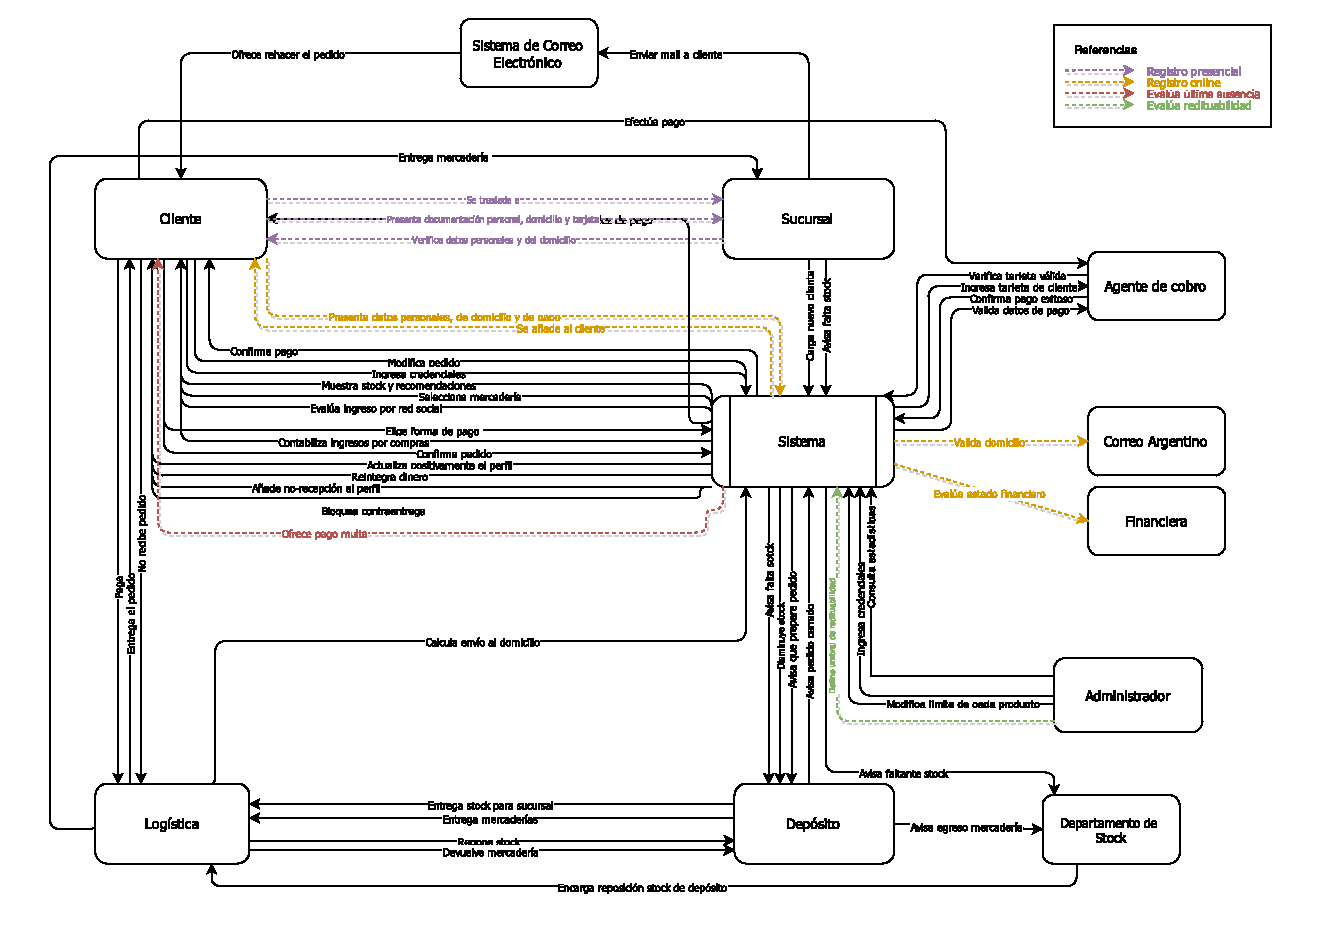
\includegraphics[width=0.9\textwidth]{tp1/images/contexto.pdf}
  \end{center}
\end{figure}


  %--
%-- Modelo de Objetivos
%--
\clearpage
\subsection{Modelo de Objetivos}

\subsubsection{Listado de objetivos}

\paragraph{1 - Objetivo primario}  \label{para:1}

El objetivo primario del sistema es revertir la disminución de ventas (1) que se
viene produciendo en la cadena de supermercados hace meses. Para ello, se nos
brinda la información de que las dos causas de las disminuciones son las largas
colas en el supermercado y el agotamiento del stock (1.3), de donde se
desprenden los objetivos (1.1) y (1.2).

\paragraph{1.1 - Reducción de colas} \label{para:1.1}

Dentro del contexto de la reducción de colas, se tomó la presunción de que cada
venta online estaría disminuyendo las colas en la sucursal (1.1.2), dado que de
este modo ese cliente, que normalmente estaría haciendo cola en el supermercado,
puede encargar los productos desde la comodidad de su casa. De este modo, se
toma el objetivo de permitir que el usuario compre de forma online (1.1.1).

\paragraph{1.1.1 - Permitir al usuario la compra online} \label{para:1.1.1}

Consideramos que para permitir que el cliente compre un pedido de forma online,
deben ocurrir dos cosas, lograr que el cliente encargue el pedido (1.1.1.1)
\footnote{lo cual incluye todo el proceso desde que el cliente se registra en
el sitio, realizando la selección de productos, acordando una fecha de entrega y
eligiendo una forma de pago}, y lograr que el pedido sea cerrado y finalizado
(1.1.1.2), que comienza con la confirmación del pedido por parte del cliente, y
culmina con la entrega del pedido (o la cancelación/anulación, según el caso).

\clearpage
\paragraph{1.1.1.1 - Lograr[Cliente encarga pedido]} \label{para:1.1.1.1}

Para que un cliente encargue un pedido, es necesario que el mismo pueda
identificarse en el sistema (1.1.1.1.1), que el pedido sea armado (1.1.1.1.2),
que se pueda acordar una fecha de entrega (1.1.1.1.3), una forma de pago
(1.1.1.1.4) y que si esta última es online, se le pueda cobrar.

\paragraph{1.1.1.1.1 - Lograr[Cliente identificado]} \label{para:1.1.1.1.1}

Para que el cliente pueda ser identificado por el sistema, es necesario que se
encuentre registrado (1.1.1.1.1.1), y que se autentique (1.1.1.1.1.2)

\paragraph{1.1.1.1.1.1 - Lograr[Cliente registrado]} \label{para:1.1.1.1.1.1}

La forma en que un cliente se registra es uno de los o-refinamientos
propuestos. Dividimos el registro entre online y presencial. El registro
online implica que el cliente se conecte al sitio, cargando sus datos
personales, y sus datos de pago, los cuales son verificados por el sistema al
momento de la registración. El registro presencial, en cambio, requiere que el
cliente se dirija a la sucursal con la documentación necesaria para verificar
identidad, domicilio y datos de pago, los cuales son archivados y verificados
por un empleado de la sucursal, y posteriormente cargados al sistema. Más
pormenores sobre este refinamiento, junto con la justificación del puntaje
asignado a los objetivos blandos, están explicados posteriormente.

\paragraph{1.1.1.1.1.2 - Lograr[Cliente se autentica de forma segura]} \label{para:1.1.1.1.1.2}

La autenticación requiere que el cliente ingrese sus credenciales
(1.1.1.1.1.2.1). Por otro lado, también es necesario proveer una interfaz que
cuente con los mecanismos de seguridad adecuados (1.1.1.1.1.2.2), por ejemplo
conexión HTTPS.

\paragraph{1.1.1.1.2 - Lograr[Armado de pedido]} \label{para:1.1.1.1.2}

Para que el pedido sea armado, consideramos que es necesario que el cliente
pueda ver el stock disponible para cada producto (1.1.1.1.2.1), y que logre
seleccionar la mercadería adecuada (1.1.1.1.2.3). Para ello, planteamos el
objetivo de mostrar recomendaciones personalizadas para cada cliente
(1.1.1.1.2.2), de acuerdo a su similaridad con otros clientes en función del
historial de compras y la edad.

\paragraph{1.1.1.1.3 - Lograr[Acordar fecha de entrega]} \label{para:1.1.1.1.3}

En el transcurso del armado del pedido, es necesario que el cliente acuerde una
fecha de entrega. Para ello, es necesario que el sistema le ofrezca un rango de
fechas disponibles (1.1.1.1.3.2), las cuales serán calculadas e informadas por
la API de logística (1.1.1.1.3.1).

\paragraph{1.1.1.1.4 - Lograr[Acordar forma de pago]} \label{para:1.1.1.1.4}

Además de que el cliente seleccione la fecha de entrega, es necesario que
acuerde con el sistema una forma de pago. Para ello, el sistema deberá informar
al cliente cuales son las formas de pago que tiene disponibles (1.1.1.1.4.2), y
el cliente deberá elegir entonces la que le resulte de su conveniencia
(1.1.1.1.4.3). Hay un o-refinamiento aquí, sobre el objetivo de evaluar si se
deberá permitir la contraentrega.

\paragraph{1.1.1.1.4.1 - Lograr[Evaluar si permitir contraentrega]} \label{para:1.1.1.1.4.1}

Para evaluar si el cliente puede realizar un pedido por contrareembolso,
proponemos dos opciones.

La primera de ellas es un límite de entregas fallidas (1.1.1.1.4.1.1), contenido
dentro de la programación del sistema, e instanciado en 1 en nuestros ejemplos,
es decir, se limita la posibilidad de que el cliente no esté presente en la
última entrega. Llegado tal caso, se le bloqueará la modalidad contraentrega
(1.1.1.1.4.1.1.1) y se ofrecerá el pago de una multa (1.1.1.1.4.1.1.2) para
poder desbloquearla (1.1.1.1.4.1.1.3). El valor de la multa, además, no es fijo,
sino que dependerá directamente del costo del envío al domicilio de ese cliente
en particular (1.1.1.1.4.1.1.2.1.1), y el costo de la mercadería que no pudo ser
reingresada a stock (1.1.1.1.4.1.1.2.1.2). Se le ofrecerán dos modalidades de
pago, pagar en efectivo en una sucursal
(1.1.1.1.4.1.1.2.2.1) o pagar online (1.1.1.1.4.1.1.2.2.2).

La segunda opción es un límite de redituabilidad (1.1.1.1.4.1.2).
Para ello, el Administrador deberá definir previamente un umbral de
redituabilidad (1.1.1.1.4.1.2.1), el cual el sistema deberá segurarse de que sea
respetado en todo momento (1.1.1.1.4.1.2.2). En caso de que el cliente produzca
costos de tal forma que la redituabilidad se encuentre por bajo del umbral, la
contraentrega deberá bloquearse (1.1.1.1.4.1.2.2.3). Para ello, es necesario
contabilizar las ganancias (1.1.1.1.4.1.2.2.1) y costos (1.1.1.1.4.1.2.2.2)
generados por el cliente. La redituabilidad, entonces, es una relación
ganancia - costo, la cual no deberá bajar más allá del umbral definido
previamente. El pago contraentrega se habilita automáticamente si el cliente
hace nuevas compras y su redituabilidad supera el umbral.

Ambas opciones están detalladas más adelante, junto con la asignación de
puntajes a los objetivos blandos.

\paragraph{1.1.1.1.5 - Lograr[Si la forma de pago es online, cobrar]} \label{para:1.1.1.1.5}

Si el cliente elige el pago online, además, hay que cobrarle. Para ello, se
cuenta con la participación del cliente, el cual deberá validarse a través del
agente de cobro, para que el importe le sea deducido de su cuenta bancaria.

\clearpage
\paragraph{1.1.1.2 - Lograr[El pedido es finalizado y cerrado]} \label{para:1.1.1.2}

Una vez que un pedido está encargado, es necesario que el mismo sea cerrado.
Aquí pueden ocurrir dos cosas, que el usuario cancele el pedido antes de que el
mismo sea preparado (1.1.1.2.2), caso en el que el mismo se anula y se le
devuelve el dinero, o que el usuario confirme el pedido (1.1.1.2.1). En este
último caso, será necesario preparar el pedido (1.1.1.2.1.1) a la vez que el
stock es restado del conteo del sistema (1.1.1.2.1.2), y luego lograr que el
mismo sea entregado a logística (1.1.1.2.1.3). Además de todo esto, será
necesario asegurar que el envío sea realizado (1.1.1.2.1.4).

\paragraph{1.1.1.2.1.4 - Lograr[Realizar el envío]} \label{para:1.1.1.2.1.4}

Al momento de realizar el envío, pueden ocurrir dos situaciones, o que el
cliente reciba el pedido (1.1.1.2.1.4.1), o que no lo reciba (1.1.1.2.1.4.2).
Por simplicidad, se englobaron todas las situaciones en las que el cliente puede
no recibir el pedido, en una situación ``el cliente no está presente''. Es
decir, también es este el caso cuando un cliente esta presente pero por alguna
razón se niega a recibir el pedido.

\paragraph{1.1.1.2.1.4.2 - Lograr[Realizar el envío]} \label{para:1.1.1.2.1.4.2}

En caso de que el cliente no reciba el pedido, será necesario deshacer la
operación, es decir, reintegrar el dinero de ser necesario (1.1.1.2.1.4.2.1),
marcar el pedido como no recibido en el historial del cliente (1.1.1.2.1.4.2.2),
y que logística devuelva el stock al depósito para que sea reingresado
(1.1.1.2.1.4.2.3). Esto significa que Depósito realizará la evaluación de los
productos (ya que algunos pueden haberse roto o perdido su calidad en el
transcurso del envío), y reingresará a stock los que considera que se encuentran
adecuados. Además, se le informará al cliente que su pedido no fue recibido
mediante un email, y se le ofrecerá rehacerlo (1.1.1.2.1.4.2.4).

\clearpage
\paragraph{1.2 - Mantener[Stock disponible]} \label{para:1.2}

Para mantener el stock disponible, se deberá mantener el stock disponible tanto
en las sucursales (1.2.1) como en los depósitos (1.2.2)

\paragraph{1.2.1 - Mantener[Stock disponible en sucursales]} \label{para:1.2.1}

Para mantener el stock disponible en las sucursales es necesario lograr realizar
un conteo periódico del stock en las sucursales (1.2.1.1), y encargar una
reposición por medio del sistema en cuanto el stock sea bajo (1.2.1.2). Por otro
lado, será necesario lograr que el depósito sea informado en cuanto haya un
pedido nuevo (1.2.1.3). Respecto a esto, la idea es que el depósito mantenga un
sistema interno propio que cuente con acceso a la misma base de datos que el
sistema web. Tamibén es necesario armar el pedido, y entregarlo a logística
(1.2.1.4), de esto se encargaría el depósito. Finalmente, logística debe
entregar la reposición de stock a la sucursal (1.2.1.5).

\paragraph{1.2.2 - Mantener[Stock disponible en depósitos]} \label{para:1.2.2}

Para poder mantener el stock en el depósito, es necesario contar con un límite
mínimo de productos, de forma tal de asegurarse de que cada producto se
encuentre siempre por encima de este límite (1.2.2.2). Como cada producto es
distinto del otro, y tienen distintos ritmos de ventas, este límite no puede ser
igual para todos los productos, ni puede estar contenido dentro del código del
programa. Para determinar este límite, entonces, será necesario contar con una
forma de modificar los productos y sus límites, según las estadísticas de ventas
de cada uno (1.2.2.1).

\paragraph{1.2.2.1 - Lograr[Modificar productos y sus límites según estadísticas]} \label{para:1.2.2.1}

Por un lado se ofrece la capacidad típica de agregar nuevos productos, modificar
los existentes, o dar de baja otros (ABM, 1.2.2.1.1). Utilizando esta interfaz,
el administrador deberá modificar los productos, estipulando el límite inferior
de stock para cada uno de ellos (1.2.2.1.3). Para ayudarlo, el sistema le ofrece
estadísticas elaboradas sobre el registro de cada transacción de los clientes.

\paragraph{1.2.2.2 - Mantener [Stock de cada producto por encima de límite estipulado por empresa]} \label{para:1.2.2.2}

El sistema monitorea constantemente el stock de cada producto, y cuando uno de
estos desciende por debajo del límite estipulado, se inicia un proceso de
reabastecimiento. Como el producto no está en suficiente cantidad en nuestros
depósitos, es necesario recurrir al Departamento de Stock (1.2.2.2.1) que se
encarga de conseguir el producto a través de los distintos proveedores. Luego se
inicia un proceso logístico que culmina con el producto en el depósito
(1.2.2.2.3), y el nuevo stock ingresado al sistema (1.2.2.2.4).

%--
%-- Modelo de objetivos - Diagramas
%--
\subsubsection{Diagramas de Objetivos}

\begin{figure}[H]\begin{center}
  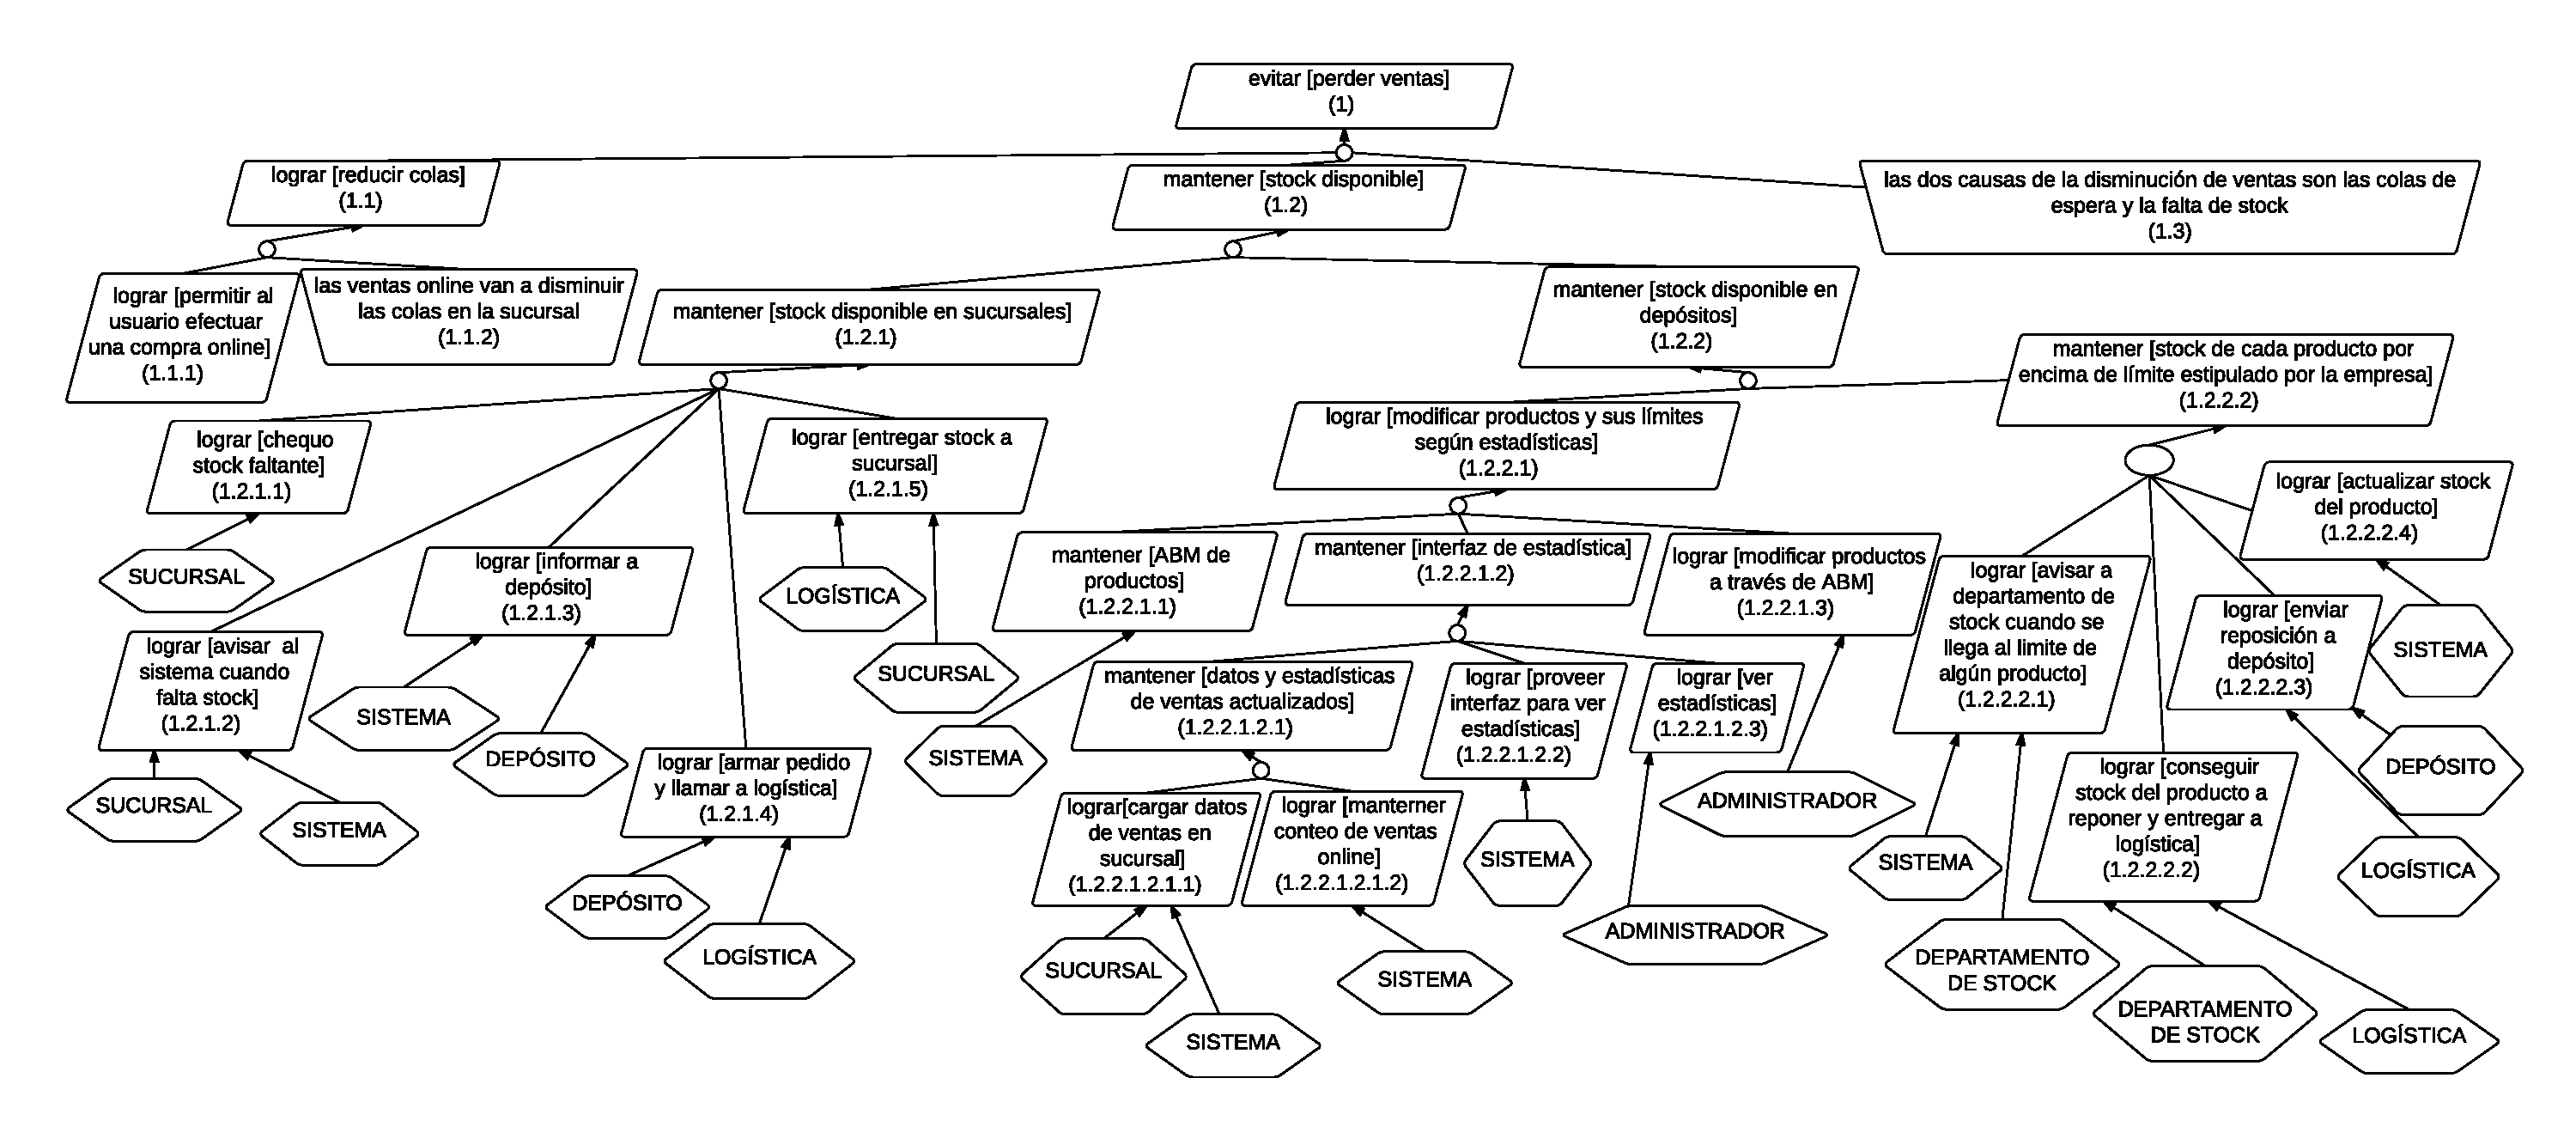
\includegraphics[angle=90,height=.9\textheight]{tp1/images/objetivos-raiz.pdf}
  \caption{Objetivo: Evitar perder ventas}
\end{center}\end{figure}

\begin{figure}[H]\begin{center}
  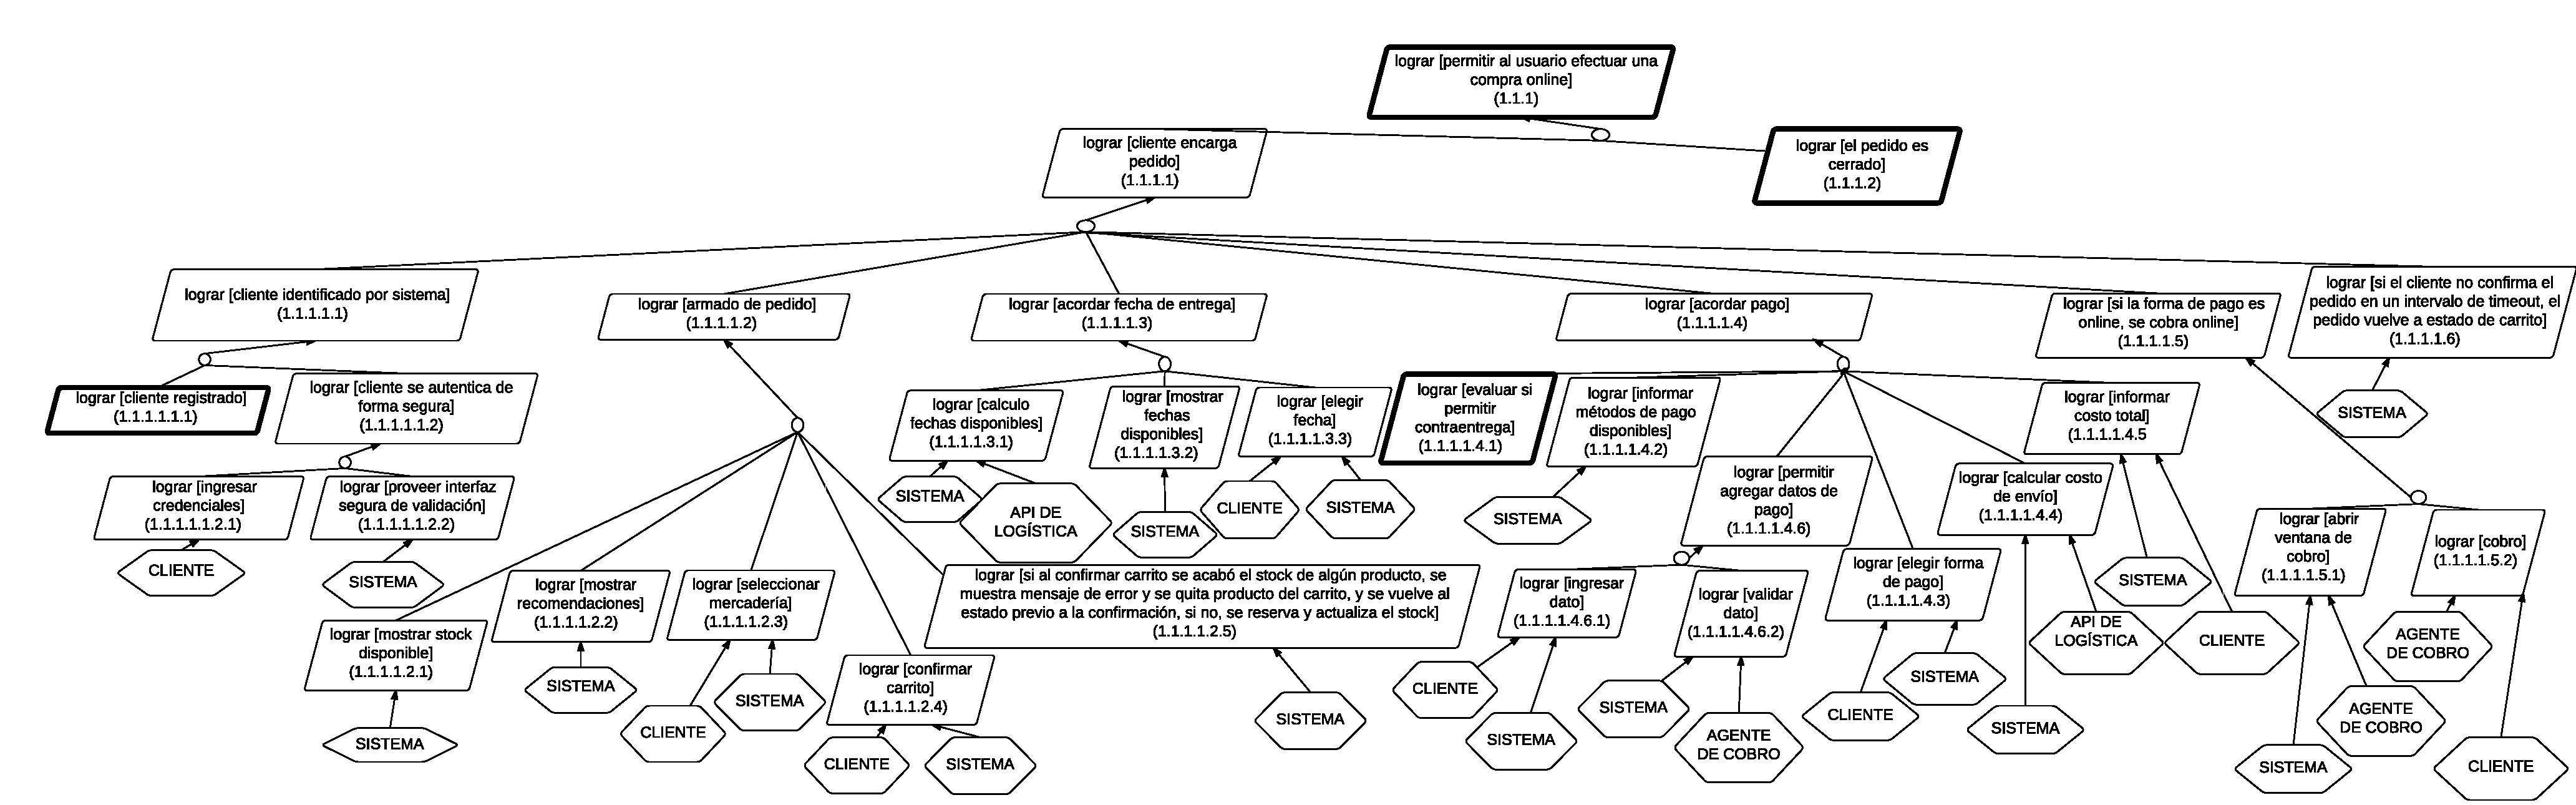
\includegraphics[angle=90,height=.9\textheight]{tp1/images/objetivos-operacion-online.pdf}
  \caption{Objetivo: Lograr permitir al usuario efectuar una compra online}
\end{center}\end{figure}

\begin{figure}[H]\begin{center}
  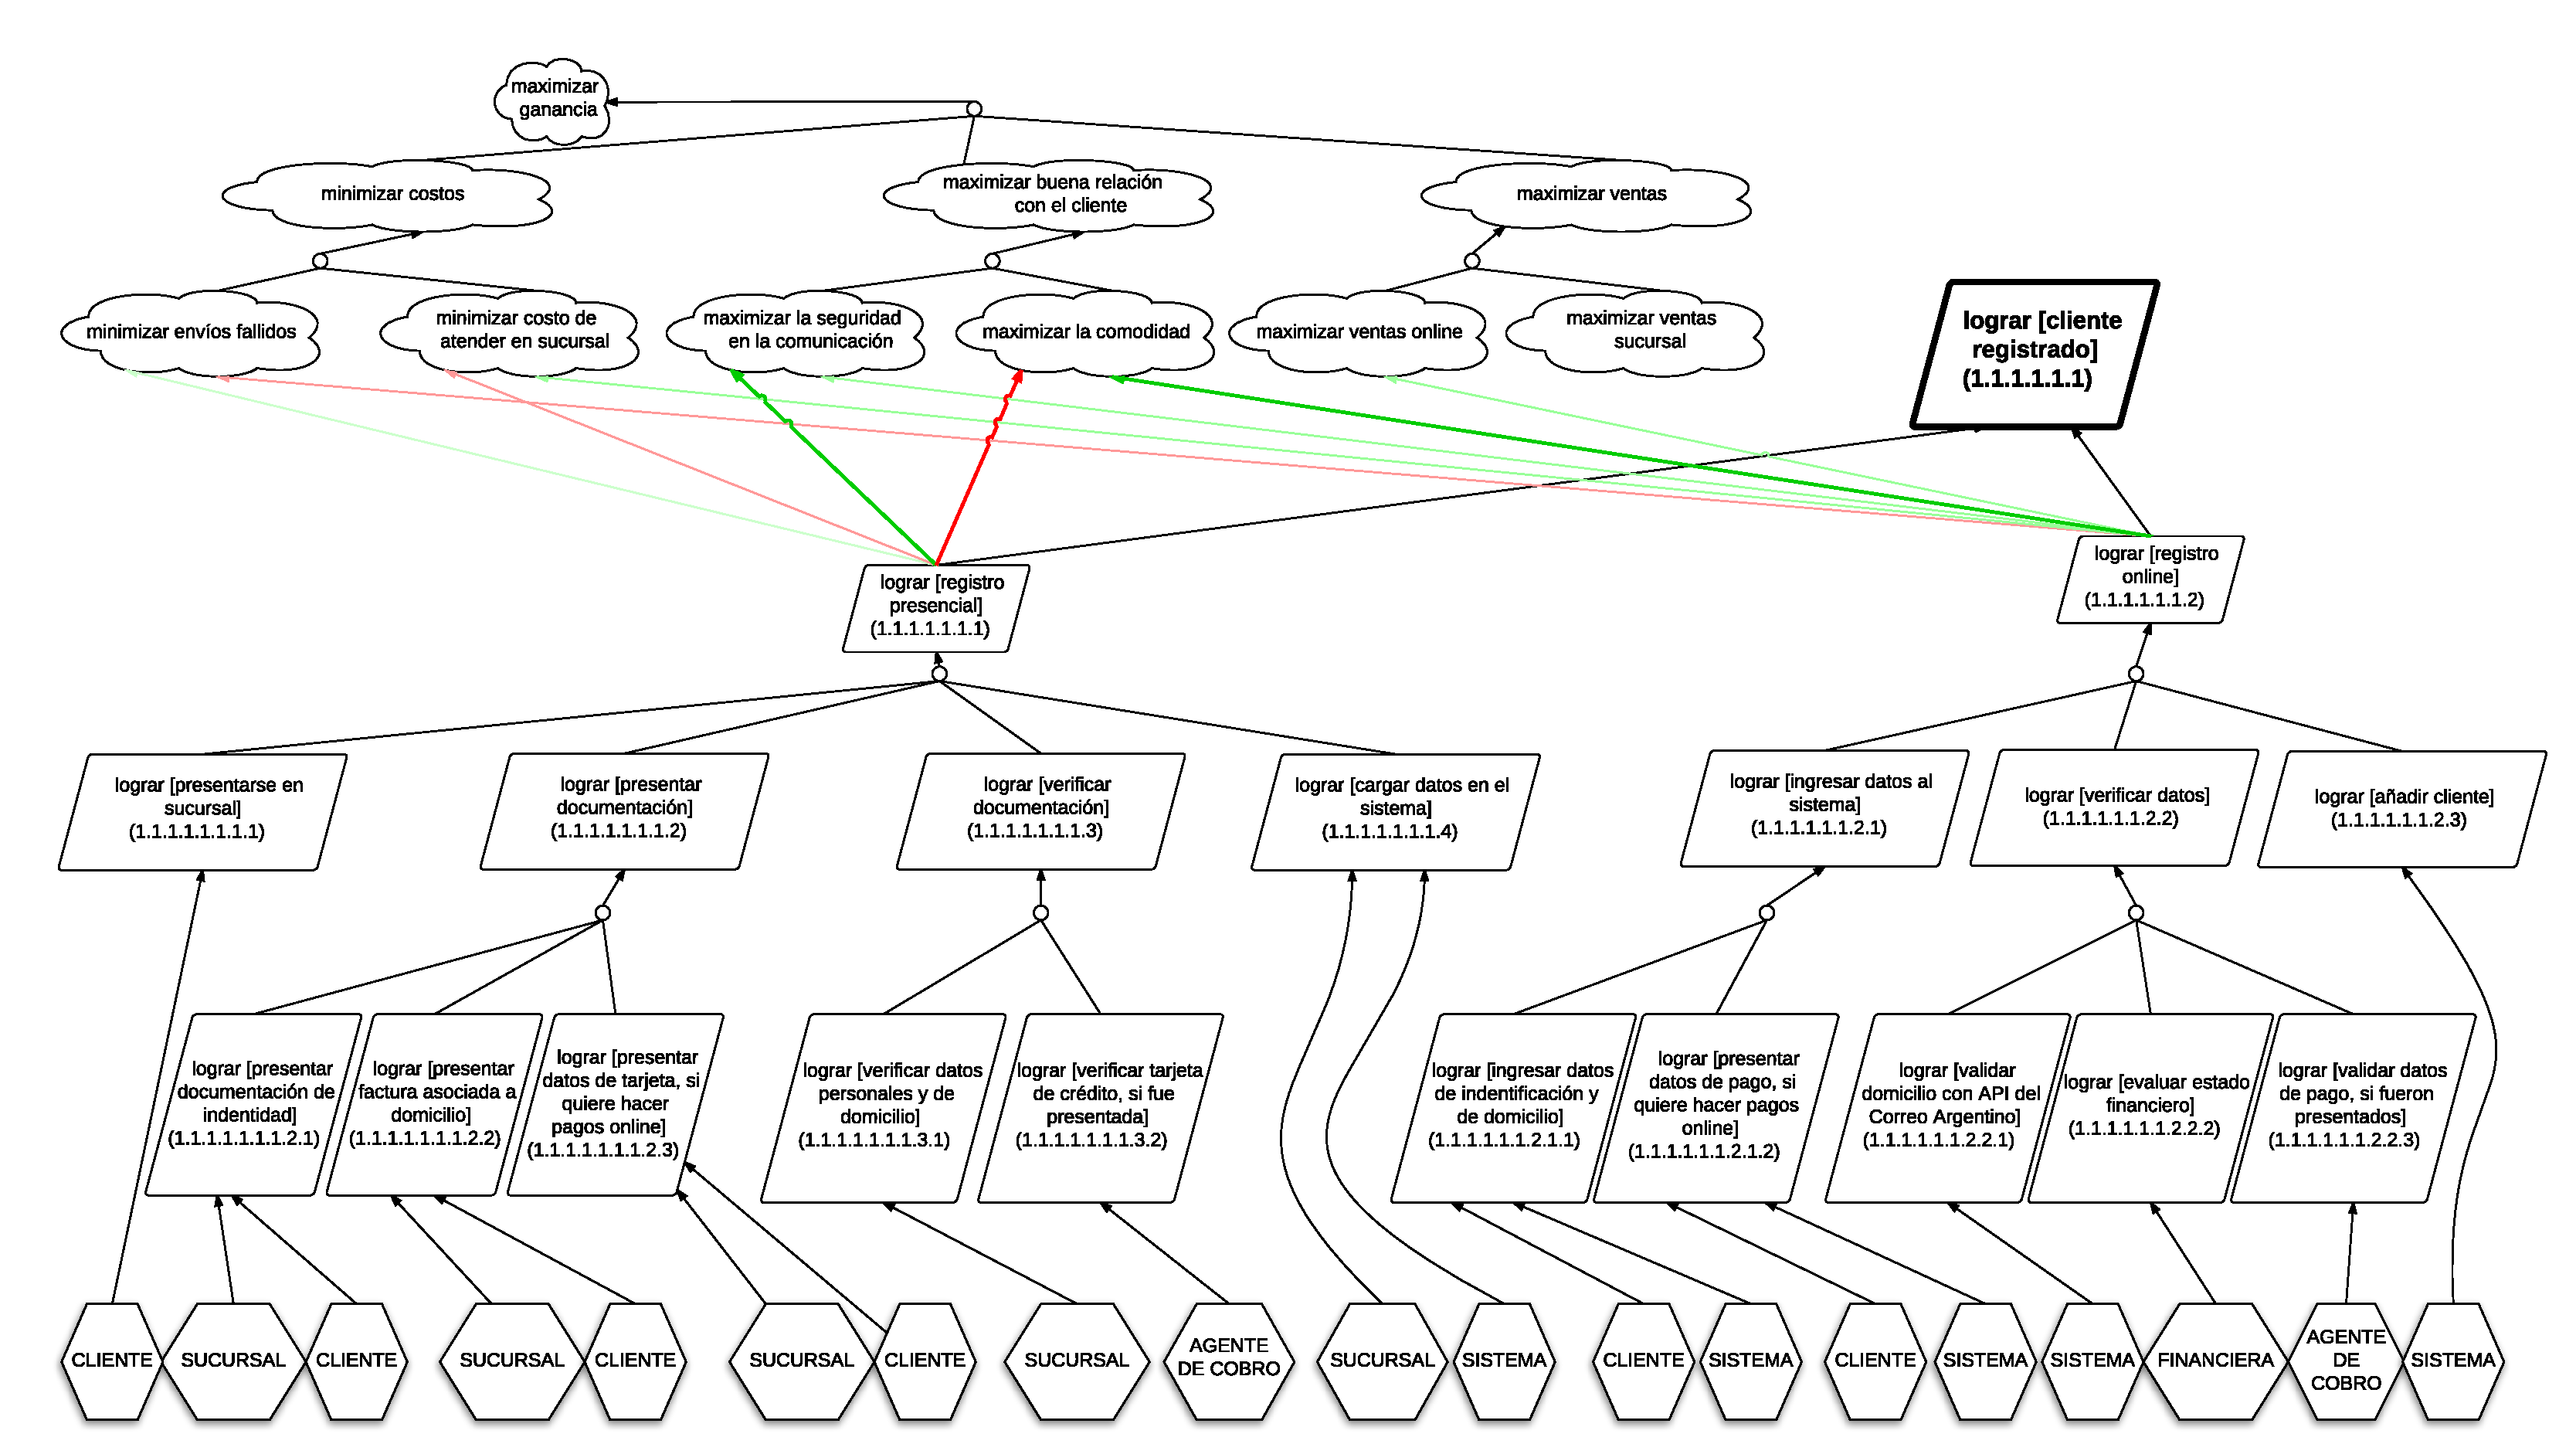
\includegraphics[angle=90,height=.9\textheight]{tp1/images/objetivos-cliente-registrado.pdf}
  \caption{Objetivo: Lograr cliente registrado}
\end{center}\end{figure}

\begin{figure}[H]\begin{center}
  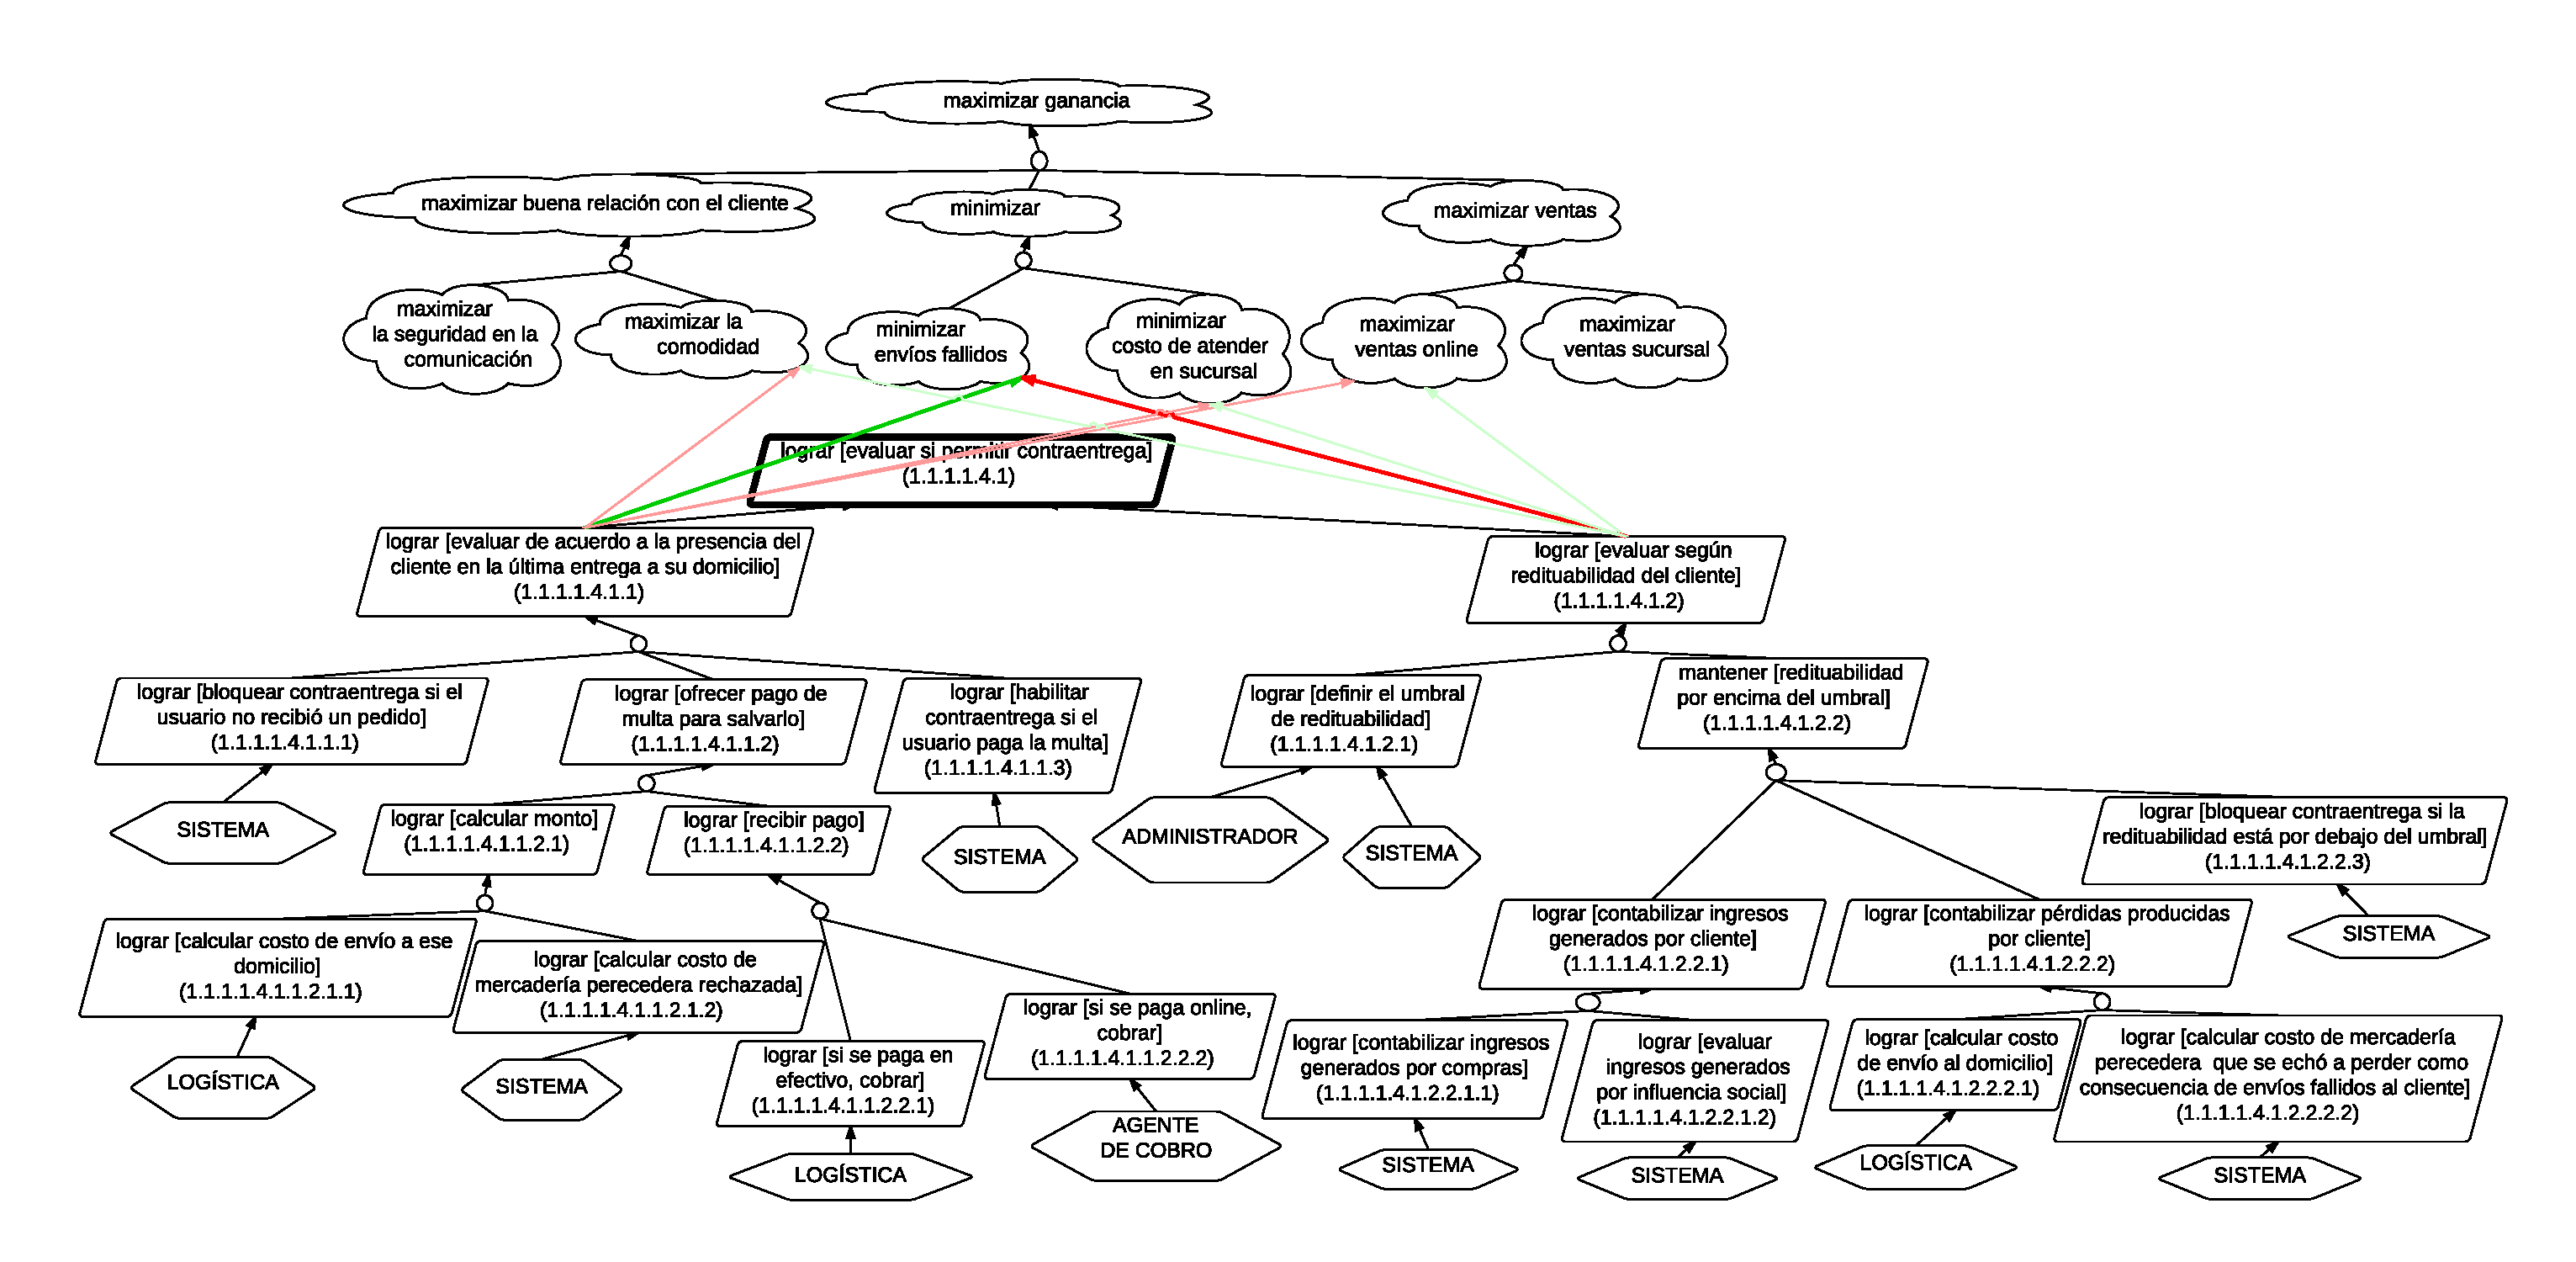
\includegraphics[angle=90,height=.9\textheight]{tp1/images/objetivos-permitir-contraentrega.pdf}
  \caption{Objetivo: Lograr evaluar si permitir contraentrega}
\end{center}\end{figure}

\begin{figure}[H]\begin{center}
  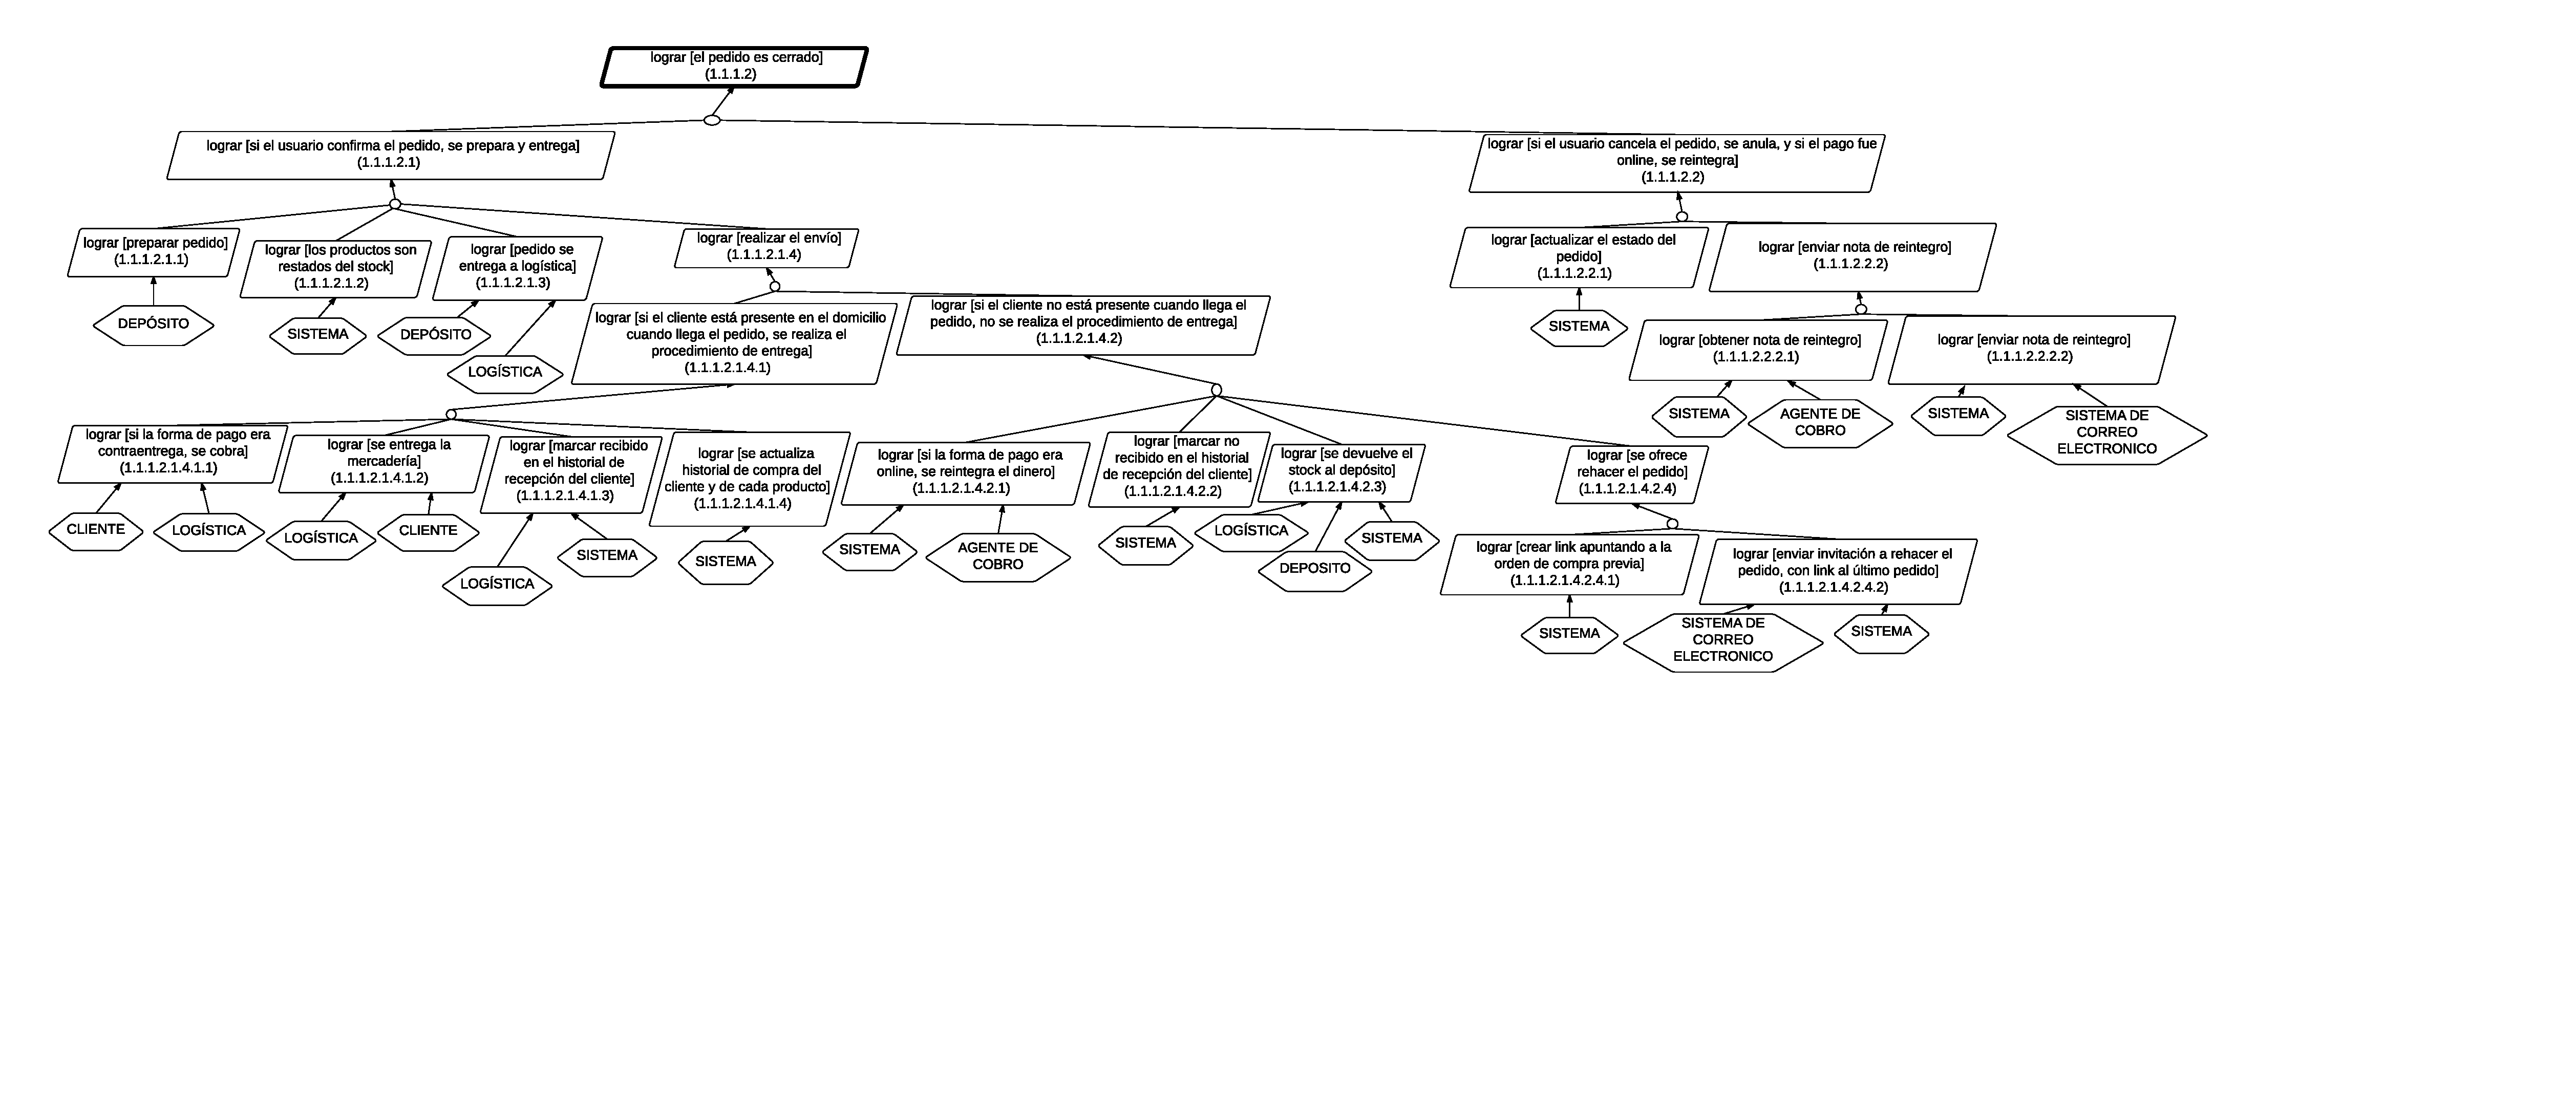
\includegraphics[angle=90,height=.9\textheight]{tp1/images/objetivos-cerrar-pedido.pdf}
  \caption{Objetivo: Lograr el pedido es cerrado}
\end{center}\end{figure}


  %--
%-- Escenarios de uso
%--
\newpage
\subsection{Escenarios representativos de uso}

%-- Escenario 1
\subsubsection{A: Registro online}

\textbf{\emph{Alice}} no es cliente habitual de la cadena mesporciento, ya que
le queda lejos de su casa como para ir caminando. Tras enterarse de la nueva
posibilidad de comprar online, se conecta al sitio web www.mesporciento.com a
través de su computadora, y registra un nuevo usuario
``\texttt{alice\_gatita93}'', ingresando para ello sus \textbf{datos
personales}, tales como nombre, domicilio, teléfono, email, y una
\textbf{contraseña segura}. El sitio verifica que los datos ingresados son
correctos, y luego le envía un mail de confirmación con un vínculo en el que
\textbf{\emph{Alice}} presiona para validar su cuenta. \textbf{\emph{Alice}}
entonces reingresa al sitio, utilizando ahora su nuevo usuario.

%-- Escenario 2
\subsubsection{B: Registro presencial con sistema de reputación}

\textbf{\emph{Bob}} es cliente habitual de la cadena mesporciento, y aprovecha
una de sus rutinarias compras para registrar su usuario en su sitio web. Para
ello, se encargó previamente de juntar la documentación requerida para el
registro: el documento de identidad, y una acreditación de domicilio, en
particular lleva la última factura de luz. Luego de las compras, le pregunta a
la cajera en dónde debe registrarse, y le indican que se dirija a la sección de
informes.

En la sección de informes no hay nadie, por lo que \textbf{\emph{Bob}} debe
esperar unos 10 minutos hasta que aparezca la encargada. Esta le pide la
documentación, y la verifica mientras le entrega a \textbf{\emph{Bob}} un
cuestionario de datos personales para que lo complete. Luego,
\textbf{\emph{Bob}} le entrega el cuestionario, y la empleada verifica que los
datos del cuestionario y la documentación coincidan. Entonces, le saca
fotocopias a la documentación y al cuestionario. Le entrega la fotocopia del
cuestionario a \textbf{\emph{Bob}}, mientras que la fotocopia de la
documentación es archivada junto con el cuestionario en un sobre de papel
madera, que a su vez es apilado junto a muchos otros sobres de aspecto similar.
Finalmente, le informa a \textbf{\emph{Bob}} que se le avisará por mail en
cuanto el registro se encuentre completo, y allí mismo le brindarán las
instrucciones para acceder al sitio.

Luego de dos semanas, \textbf{\emph{Bob}} recibe un email de parte del remitente
felicitaciones@mesporciento.com, y asunto <<Bienvenido a una nueva forma de
comprar>>, en el que se le informa que ya se encuentra habilitado su usuario
``\texttt{marley\_b420}''

%-- Escenario 3
\subsubsection{C: Pago online}

\textbf{\emph{Charlie}} se conecta a la web de mesporciento desde su tablet, con
su usuario ``\texttt{je\_suis\_moi}'', dispuesto a iniciar su compra de
productos semanal, de forma online. Para ello, revisa el listado de productos, y
agrega a su \textbf{carrito virtual} los que necesita. Una vez que el carrito
contiene todos los productos que desea, presiona el botón \texttt{``FINALIZAR
COMPRA''}, el cual lo dirige a la pantalla de cierre de pedido. En esta
pantalla, se le informa del costo total de la compra, y se le ofrecen opciones
de fechas y horarios posibles de entrega, de entre las que
\textbf{\emph{Charlie}} elige el Miércoles de la semana que viene, por la
mañana, ya que sabe que en ese horario va a estar en su casa.

Luego, en la siguiente pantalla, elige la opción de Pago Online, y el sitio le
solicita que elija un método de pago de entre las distintas opciones
disponibles. Ya que \textbf{\emph{Charlie}} confía mucho en el sistema
\texttt{PayPal} (como ejemplo de Agente de Cobro), lo elige, tras lo cual se abre una ventana externa que redirige
al sitio de PayPal, en que tras ingresar su usuario y su clave se le solicita
confirmar el valor de la compra. Luego de que esta ventana se cierra, el sitio
le muestra una animación muy jocosa de un tigre mirando un reloj, mientras
debajo se puede leer la frase \texttt{``Por favor, espere, estamos validando el
pago...''}. Tras unos segundos, el tigre comienza a bailar, el mensaje se
desvanece, y lo reemplaza un nuevo mensaje \texttt{``Su pago se encuentra
confirmado. Le hemos enviado un mail con la información de su pedido. Gracias
por confiar en nosotros. En unos instantes, será redirigido a la página
principal.''}.

%-- Escenario 4
\subsubsection{D: Pago contrareembolso}

\textbf{\emph{Dave}} tiene un problema de adicción al casino. Normalmente, con
la ayuda de sus amigos y familiares, lo controla sin mayores inconvenientes.
Pero hace 1 semana tuvo un viaje laboral, y en el último día, libre para todos
los empleados, no resistió la tentación de jugar una o dos tiradas de ruleta,
con el efectivo que llevaba encima. Tuvo la mala suerte de que le fue
relativamente bien, ganó ambas jugadas lo que le hizo cuadruplicar su efectivo.
Envalentonado por su repentino y misterioso golpe de suerte, se dirigió a la
casilla de venta de fichas, y gastó todo el dinero de su cuenta bancaria en
fichas. También compró fichas con su tarjeta de crédito, en un pago, hasta
alcanzar el límite. Compró en total 450 fichas, y volvió a dirigirse a la
ruleta. Su plan inicial era realizar una paciente Martingala, pero un rayo
cósmico atravesó su mente momentos antes de colocar la apuesta, y supo entonces
que debía elegir el número 7. Claro, porque este era el séptimo día del viaje
laboral, y había tenido mucha suerte, por lo que el siete era un buen número.
Claramente, \textbf{\emph{Dave}} perdió todo su dinero, y no solo eso, sino que
se endeudó gravemente, saturando el límite de su tarjeta de crédito.

Al volver a su casa, le cuenta lo sucedido a su tío, pidiéndole que no le cuente
a nadie, y este le presta dinero ``hasta que logre salir de la situación''. Como
no tiene tiempo de ir al supermercado, ya que debe hacer horas extras para pagar
sus deudas, aprovecha el sistema de compras online de mesporciento para encargar
las provisiones de la semana durante la noche. Se autentica en el sitio con su
usuario, ``\texttt{lucky\_guy\_00}'', elige los productos indispensables para el
resto del mes, y pacta una fecha de entrega para el día siguiente. Al momento de
elegir la opción de pago, advierte que no puede realizar un pago online, ya que
la tarjeta se encuentra saturada, por lo que opta por elegir la opción de pago
contrareembolso.

Al otro día, temprano, suena el timbre, y recibe el pedido, el cual paga en
efectivo, y les deja una modesta propina a los muchachos para que carguen las
bolsas hasta la cocina de su casa.

%-- Escenario 5
\subsubsection{E: Entrega correcta}

El Martes 13 de Abril \textbf{\emph{Erin}} realizó un pedido de torta de
cumpleaños, cotillón y un regalo grandioso para ser entregado el Martes
siguiente, en conmemoración del 50-cumpleaños de su tía. Aprovecha la
posibilidad para elegir que su pedido sea entregado en la casa de su tía, y no
en su domicilio. Para ello, intenta modificar el domicilio de su usuario
``\texttt{ireland\_green}'', pero el sistema no se lo permite. Entonces, como
\textbf{\emph{Erin}} es muy inteligente, crea un nuevo usuario
``\texttt{tia\_50}'', especial para esta ocasión, el cual completa con los datos
de su tía. Por comodidad, además, lo paga en línea, con una tarjeta de crédito
(la suya, no la de su tía), ya que por costumbre familiar está prohibido hablar
de dinero durante el cumpleaños de una tía, y quiere evitar malos momentos
durante el episodio festivo.

Llegado el día, están todos festejando, ya con algunas copitas encima, cuando la
tía grita a \textbf{\emph{Erin}}: <<¿y la torta? ¿y los juguetitos que me habías
prometido?>>. En ese instante, justamente, suena el timbre, y resultan ser los
empleados de mesporciento. \textbf{\emph{Erin}} les abre la puerta y les indica
dónde dejar la mercadería. Les dice que no puede darles propina por una
costumbre familiar, tras lo cual los empleados regresan a su camión,
apesadumbrados.

%-- Escenario 6
\subsubsection{F: Ausente durante entrega con límite de entregas fallidas fijo}

\textbf{\emph{Frank}} es una persona muy olvidadiza. Tanto es así, que durante
la mañana de hoy, fue hasta el banco a cobrar un cheque, para terminar dándose
cuenta que no lo había llevado. No fue sino hasta la mañana del día siguiente,
al leer su email, que se enteró que, durante su ausencia en el banco, había
recibido una visita del supermercado Mes\%, al cual había justamente encargado
una compra el día anterior. Utilizando un vínculo provisto dentro del mismo
mensaje, programó la visita para ese mismo día, al mediodía, y luego se ató un
piolín en el dedo corazón para recordarlo. Entonces miró un poco de televisión,
y tras terminar el programa, cuando se dispuso a cambiar de canal, se dio cuenta
que su dedo, el del piolín obviamente, estaba totalmente ennegrecido y arrugado.
Peor aún, a pesar de desatarlo, este había perdido la sensibilidad, y no
recuperaba su rosadito color habitual. \textbf{\emph{Frank}} se asustó tanto,
que corrió raudo hasta la calle, y tomó un taxi hasta el hospital más cercano,
sin advertir que estaba en pijama, y que este no dejaba nada a la imaginación.
En el hospital, les explicó que, por razones que no podemos repetir, para él era
muy importante este dedo, y que no podía perderlo. Entonces le dieron una bata
para que pueda poner sobre el pijama y proteger la sensibilidad del resto de los
pacientes, y le realizaron estrambóticos procedimientos médicos. Luego de un par
de horas \textbf{\emph{Frank}} pudo recuperar el funcionamiento habitual de su
dedo. Cuando el médico le preguntó que por qué se le había puesto así el dedo,
\textbf{\emph{Frank}} le explicó que se había atado algo. Tras lo cual el médico
hizo una obvia segunda pregunta, lo cual provocó algo similar a un click en
algún recóndito lugar del cerebro de \textbf{\emph{Frank}}, seguido de una
catarata de imágenes mentales, la mayoría de ellas relacionadas al supermercado
Mes\%. Entonces, repentinamente, se levantó, corrió hasta la puerta del
hospital, y tomó un taxi nuevamente hasta su casa. Al llegar, abrió su mail,
para enterarse de que nuevamente había perdido la entrega. Se le informaba,
además, de que su usuario ``\texttt{f\_estein}'' había perdido la posibilidad de
realizar compras contrareembolso, hasta pagar una multa de \$100, lo cual
ciertamente lo puso de muy mal humor.

\subsubsection{G: Cancelación de pedido}

\textbf{\emph{Gabriel}} había hecho un pedido el lunes a la mañana, pagándolo con tarjeta de crédito. A la tarde
descubre mejores precios en los chinos de la vuelta, y decide cancelar la compra
para hacerla en ese lugar que le resulta más económico (haciendo las cuentas,
llega a la conclusión de que con la diferencia podía comprar un videojuego para
sus hijos). Entonces, vuelve rápido de los chinos a su casa, y entusiasmado
chequea que aún pueda hacer la cancelación. Para ello ingresa al sitio
\texttt{www.mesporciento.com} con su cuenta ``\texttt{gabi\_25x8}'', poniendo su
contraseña, y luego seleccionando el pedido vigente. Selecciona la opción de
modificación de pedido y posteriormente, al comprobar que no está cerrado, lo
cancela.

El sistema le confirma la cancelación y se le hace una nota de crédito para
reintegrarle el dinero. Finalmente  \textbf{\emph{Gabriel}} vuelve contento a
los chinos a hacer la compra y con lo que le sobra, compra el videojuego para
sus hijos (¡aunque como padre responsable, primero lo juega el para enseñarle a
ellos!).

\subsubsection{H: Modificación de pedido.}

En la casa de \textbf{\emph{Helena}} van a festejar la navidad. Unas horas
después de que hacer un pedido con la mercadería necesaria para preparar la
cena, su esposo \textbf{\emph{Horacio}} le comenta que habían sido invitados a
la cena su vecina \textbf{\emph{Hermenegilda}}, junto con sus hijos, debido a
que el marido y los parientes de esta aún no habían regresado del exterior, ya
que se encontraban en un viaje por asuntos laborales. Por este motivo,
\textbf{\emph{Helena}} decide modificar el pedido que tenía hecho, incrementando
la cantidad de productos comprados (como por ejemplo las gaseosas). Para ello,
ingresa al sitio \texttt{www.mesporciento.com} validando los datos de su cuenta,
y chequea que aún no haya sido cerrado dicho pedido. Al comprobarlo, selecciona
la opción para modificarlo, y agrega la mercadería que desea. Luego selecciona
contrareembolso como opción de pago, y sistema le confirma la modificación. Dado
que el pedido había sido originalmente pagado de forma online,
\textbf{\emph{Helena}} deberá abonar la diferencia en efectivo en cuanto lo
reciba.


\subsection{I: Preparar y cerrar pedido}

\textbf{\emph{Ismael}}, un empleado del depósito, entra al sistema interno y
revisa los pedidos pendientes. Selecciona el primero de la lista (están
ordenados por prioridad) y lo prepara poniendo en una caja los productos
encargados. Luego lo cierra en el sistema interno.


\subsection{J: Alarma y reposición por bajo stock en depósitos}

Luego de que una clienta comprara diez packs de gaseosas Coca-Cola, se agotó el
stock de dicho producto, por lo que saltó  la alarma del sistema. El sistema
entonces le avisa al Departamento de Stock de forma automática. Un superior del
Departamento de Stock recibe el aviso y hace los pedidos correspondientes a
Logística, quien finalmente se encarga de  reponer el stock.
\fixme[arreglar]

%\subsubsection{Administración inteligente de productos de depósitos}
%\fixme[El administrador ingresa al sistema, ve estadísticas,
%modifica productos vigentes (abm)]
